\documentclass[letterpaper]{article}
%\documentclass[legalpaper]{article}
\usepackage[T1]{fontenc}
\usepackage[utf8]{inputenc}
\usepackage[spanish,es-tabla]{babel}
\usepackage[lmargin=3cm,rmargin=3cm,top=3cm,bottom=3cm]{geometry}
\usepackage{amsmath,amsfonts}
\usepackage{mathtools}
\usepackage{graphicx}
\usepackage{lipsum}
\usepackage{titling}
\usepackage{fancyhdr}
\usepackage{setspace}
\usepackage[natbibapa]{apacite}
\usepackage{caption}
\usepackage{float}
\usepackage{dirtytalk}

\lhead{Universidad del Bío-Bío\\ Facultad de ingeniería \\ Escuela de Ingeniería Industrial}
%\lhead{\begin{picture}(0,0) \put(0,0){
\includegraphics[height=10mm]{logos/escuela}} \end{picture}}
\rhead{\begin{picture}(0,0) \put(-50,0){
\includegraphics[height=10mm]{logos/escudo_ubb_2}} \end{picture}}


%\setlength{\parindent}{0pt}
\bibliographystyle{apacite}
\pagestyle{fancy}


\usepackage{titlesec}
\titleformat*{\section}{\large\bfseries\centering}
\titleformat*{\subsection}{\normalsize\bfseries}

\begin{document}
\vspace*{0.5\baselineskip}
\begin{center}
\begin{Large}
\textbf{\underline{Guía N\textsuperscript{\underline{o}}6}}
\end{Large}\\
\vspace*{0.5\baselineskip}
\textbf{Optimización Lineal} \\
\vspace*{0.5\baselineskip}
\begin{footnotesize}
\textbf{Código}: 430373\\
\textbf{Semestre}: 2019-2
\end{footnotesize}
\end{center}

\noindent \textbf{Profesor}: Dr Carlos Obreque Niñez  \hfill Ayudante: Alex Barrales Araneda\\
\noindent \textbf{Fecha}: \today

\subsection*{Problema 1}
Considere el siguiente Problema de Programación Lineal:
\begin{align*}
\mbox{Maximizar }&Z = -2X_1 - X_2\\
s.a.\\
&-X_1 + X_2 \leq 10\\
&X_1 + X_2 \geq -12\\
&X_1 \leq 1 ; X_2\: n.r.s.\\
\end{align*}

\begin{itemize}
\item Escriba el problema de PL en la Forma Estándar.
\item Determine una solución básica factible de (c) e indique en el gráfico a cual vértice corresponde.
\end{itemize}

\subsection*{Problema 2}
Considere el siguiente modelo de PL:
\begin{align*}
\mbox{Minimizar }&Z = 4X_1 + 5X_2\\
s.a.\\
&2X_1 + 5X_2 \leq 20\\
&X_1 + 2X_2 \geq -4\\
&2X_1 - 3X_2 \leq 12\\
&X_1 \geq 0 ; X_2\: n.r.s.\\
\end{align*}
\begin{itemize}
\item Obtenga la solución básica factible correspondiente a la solución óptima.
\item Determine otra solución básica factible e indique gráficamente a qué punto extremo corresponde.
\end{itemize}

\subsection*{Problema 3}
Considere el siguiente modelo de programación lineal:
\begin{align*}
\mbox{Minimizar }&Z = 2X_1 + X_2\\
s.a.\\
&-2X_1 - 3X_2 \leq 6\\
&-4X_1 + 5X_2 \leq 20\\
&5X_1 + 3X_2 \leq 15\\
&X_1\: n.r.s.; X_2 \geq 0 \\
\end{align*}
El algoritmo Simplex produce la siguiente tabla intermedia:

\centering{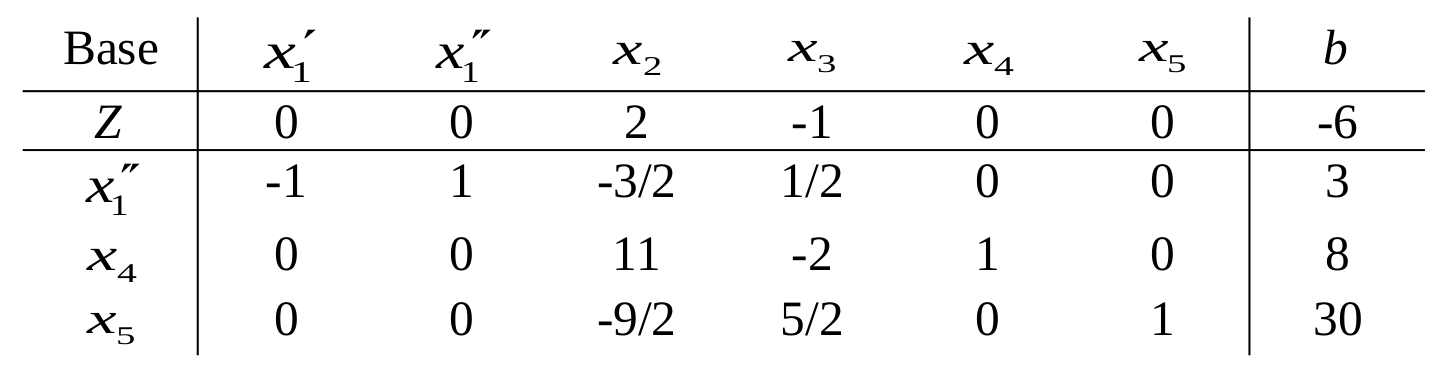
\includegraphics[width=0.6\textwidth]{images/simplex}}

\begin{itemize}
\item Indique si la solución básica factible es la óptima. En caso contrario continúe iterando hasta encontrar la solución óptima.
\end{itemize}

\subsection*{Problema 4}
Resuelva el siguiente modelo de programación lineal utilizando el algoritmo Simplex.
\begin{align*}
\mbox{Maximizar }&Z = -X_1\\
s.a.\\
&X_1 + 20 \leq X_2\\
&X_1  = 100\\
&X_2  \leq 150\\
&X_1 \geq 0 ; X_2 \geq 0\\
\end{align*}
\begin{itemize}
\item Determine la Solución Optima.
\end{itemize}
\end{document}
